\chapter{\ifproject%
\ifenglish Experimentation and Results\else การทดลองและผลลัพธ์\fi
\else%
\ifenglish System Evaluation\else การประเมินระบบ\fi
\fi}

การทดสอบเว็บแอปพลิเคชันจะแบ่งเป็น 2 หัวข้อหลักตามวัตถุประสงค์ของโครงงาน คือ การทดสอบประกาศกิจกรรมและแสดงความสนใจเข้าร่วมกิจกรรม และ ทดสอบระบบให้คะแนนกิจกรรม
โดยจะทดสอบเรื่อง การเพิ่มข้อมูลลงในฐานข้อมูลและการดึงข้อมูลจากฐานข้อมูลเพื่อแสดงผลให้กับผู้ใช้

\section{ผลทดสอบการประกาศกิจกรรมและแสดงความสนใจเข้าร่วมกิจกรรม}
\subsection{การเข้าสู่ระบบ}
ผู้ใช้สามารถเข้าสู่ระบบผ่าน Google Account ได้ แต่การเข้าสู่ระบบด้วย CMU Account ยังมีปัญหา
\begin{figure}[htb]
    \begin{minipage}[b]{0.48\textwidth}
        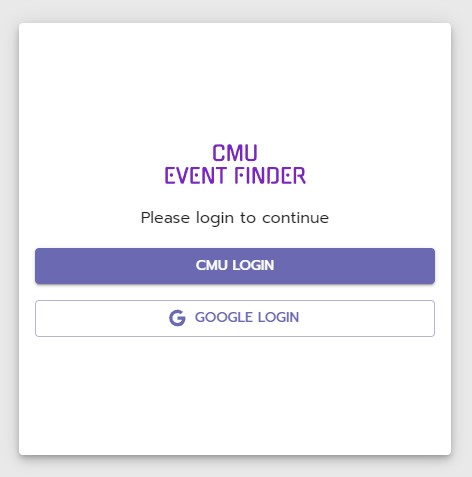
\includegraphics[width=\textwidth, height=4.5cm]{public/login-page.jpg}
        \caption[ผลทดลองหน้าเข้าสู่ระบบ]{หน้าเข้าสู่ระบบ}
    \end{minipage}
    \hfill
    \begin{minipage}[b]{0.48\textwidth}
        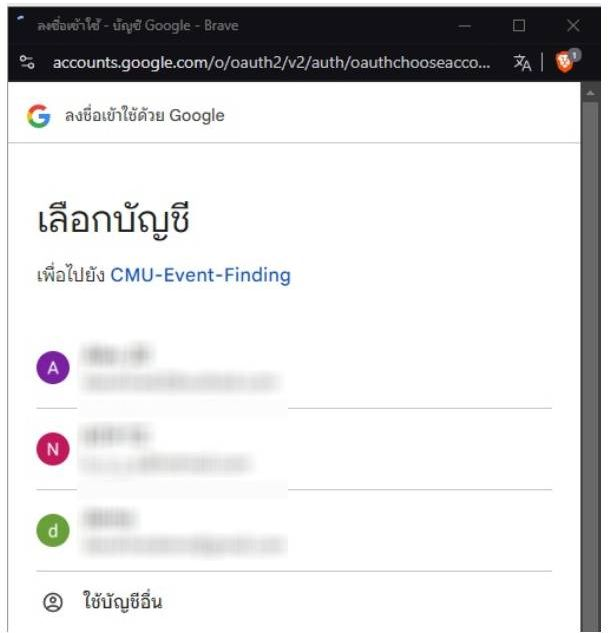
\includegraphics[width=\textwidth, height=4.5cm]{public/login-prompt.jpg}
        \caption[ผลทดลองหน้าต่างเลือก Google Account]{หน้าต่างเลือก Google Account}
    \end{minipage}
\end{figure}
\begin{figure}[H]
    \begin{center}
    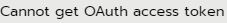
\includegraphics[scale=1]{public/cmu-bug.png}
    \end{center}
    \caption[ผลทดลองข้อผิดพลาดการเข้าสู่ระบบด้วย CMU Account]{ข้อผิดพลาดการเข้าสู่ระบบด้วย CMU Account}
    \label{fig:cmu-bug}
\end{figure}
\begin{figure}[H]
    \begin{center}
    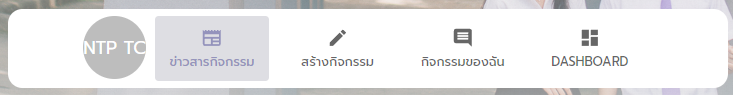
\includegraphics[scale=0.7]{public/after-login-nav.png}
    \end{center}
    \caption[ผลทดลองเมนูหลังเข้าสู่ระบบ]{เมนูหลังเข้าสู่ระบบ}
    \label{fig:after-login-nav}
\end{figure}
\clearpage
\subsection{การแสดงผลให้กับผู้ใช้ที่เข้าสู่ระบบและไม่ได้เข้าสู่ระบบ}
ผู้ใช้ที่ไม่ได้เข้าสู่ระบบสามารถดูรายละเอียดกิจกรรมที่ตนเองสนใจได้ แต่หากต้องการใช้งานระบบอื่น จะต้องเข้าสู่ระบบ
\begin{figure}[H]
    \begin{minipage}[b]{0.48\textwidth}
        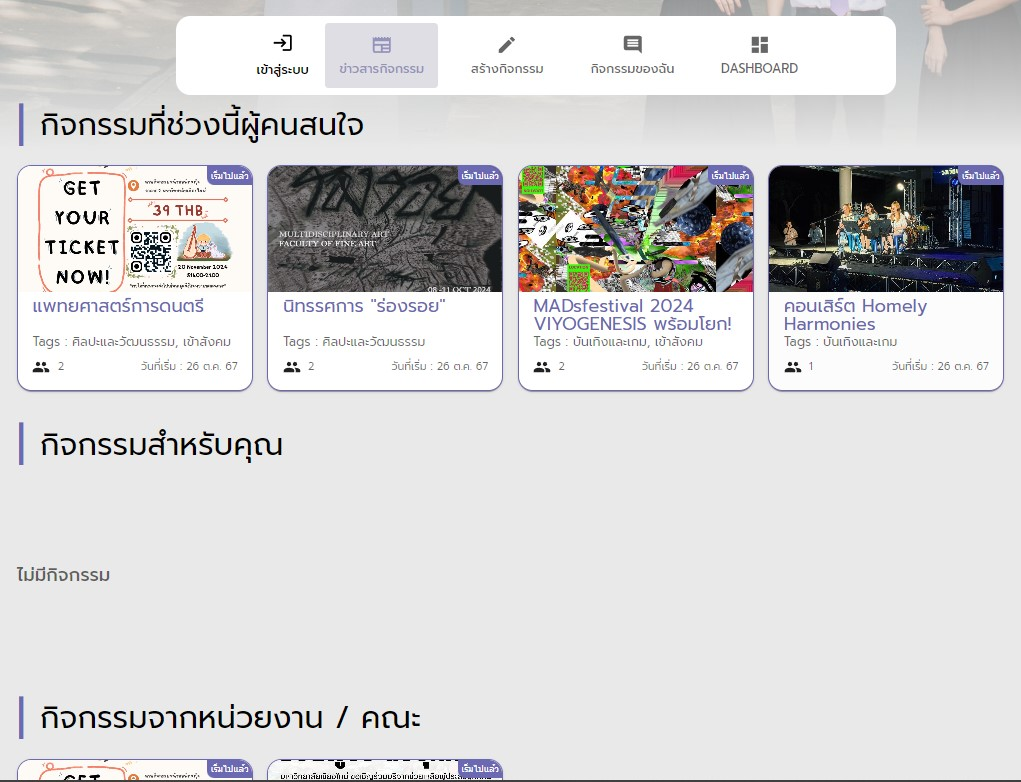
\includegraphics[width=\textwidth, height=5cm]{public/landing-nologin.jpg}
        \caption[ผลทดลองหน้าแรก(ไม่ได้เข้าสู่ระบบ)]{หน้าแรก(ไม่ได้เข้าสู่ระบบ)}
    \end{minipage}
    \hfill
    \begin{minipage}[b]{0.48\textwidth}
        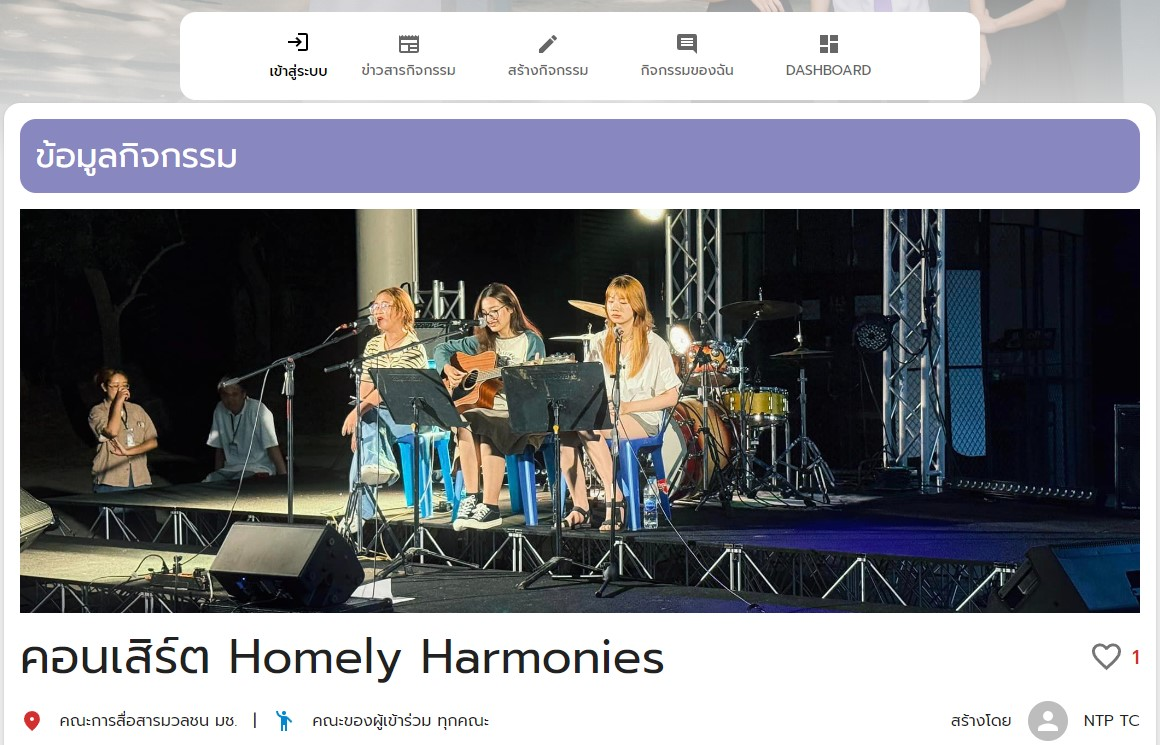
\includegraphics[width=\textwidth, height=5cm]{public/act-nologin.jpg}
        \caption[ผลทดลองหน้ารายละเอียดกิจกรรม]{หน้ารายละเอียดกิจกรรม}
    \end{minipage}
\end{figure}
\subsection{การเลือกความสนใจประเภทกิจกรรมและแนะนำกิจกรรมตามความสนใจ}
เมื่อผู้ใช้เลือกประเภทกิจกรรมที่สนใจแล้ว ส่วนกิจกรรมสำหรับคุณในหน้าแรกจะแนะนำกิจกรรมตามประเภทที่ได้เลือกไว้ โดยมีวิธีการคำนวณคือ
\begin{enumerate}
    \item ประเภทกิจกรรมที่เลือกอันดับแรก มี 3 คะแนน
    \item ประเภทกิจกรรมที่เลือกอันดับที่สอง มี 2 คะแนน
    \item ประเภทกิจกรรมที่เลือกอันดับที่สาม มี 1 คะแนน
\end{enumerate}
หากกิจกรรมใดมีประเภทกิจกรรมตรงครบทั้งสามประเภท จะได้คะแนนรวม 6 คะแนน กิจกรรมที่ไม่มีประเภทกิจกรรมตรงกับผู้ใช้จะได้ 0 คะแนน โดยกิจกรรมที่มีคะแนนมากที่สุด 4 อันดับจะถูกแนะนำให้กับผู้ใช้
\begin{figure}[H]
    \begin{center}
    \fbox{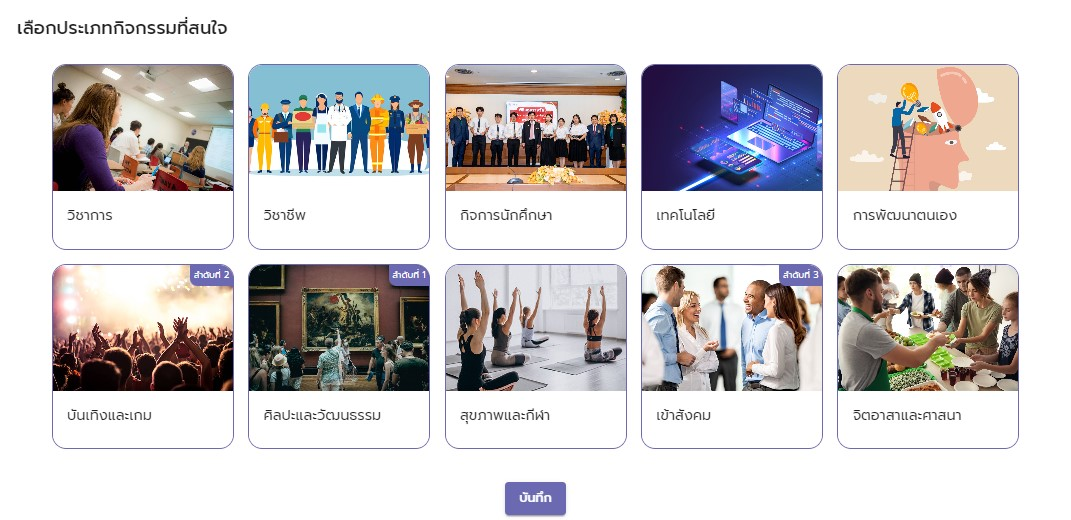
\includegraphics[scale=0.5]{public/tag-choose2.jpg}}
    \end{center}
    \caption[ผลทดลองหน้าเลือกประเภทกิจกรรมที่สนใจ]{หน้าเลือกประเภทกิจกรรมที่สนใจ}
    \label{fig:tag-choose-2}
\end{figure}
\begin{figure}[H]
    \begin{center}
    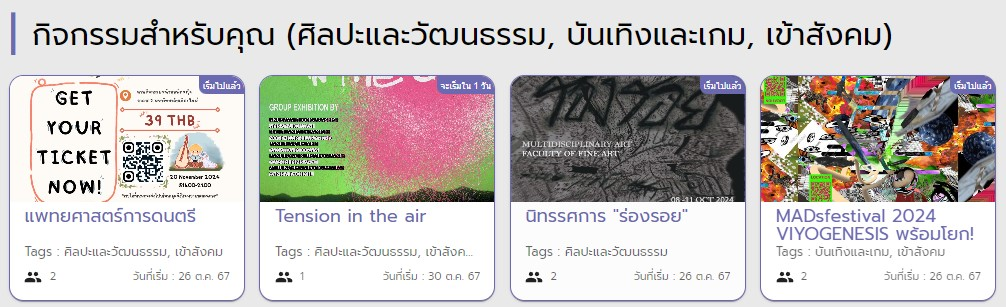
\includegraphics[scale=0.5]{public/tag-choose-result.jpg}
    \end{center}
    \caption[ผลทดลองส่วนแนะนำกิจกรรมให้กับผู้ใช้]{ส่วนแนะนำกิจกรรมให้กับผู้ใช้}
    \label{fig:tag-reccommend}
\end{figure}
% \subsection{การแนะนำกิจกรรมตามความสนใจของผู้ใช้}
\subsection{การประกาศกิจกรรม}
\subsubsection{ข้อมูลที่จำเป็นต้องกรอก}
เมื่อมาที่หน้าสร้างกิจกรรม หากผู้ใช้กดสร้างกิจกรรมโดยไม่ได้กรอกข้อมูลที่จำเป็น จะไม่สามารถสร้างกิจกรรมได้ โดยข้อมูลที่จำเป็นต้องกรอก ได้แก่
\begin{itemize}
    \item ชื่อกิจกรรม
    \item คำอธิบายกิจกรรม
    \item ประเภทกิจกรรม
    \item วันเริ่มต้น
    \item วันสิ้นสุด
    \item สถานที่จัดกิจกรรม
    \item คณะของผู้เข้าร่วม
    \item รูปภาพ
\end{itemize}
\begin{figure}[H]
    \begin{center}
    \fbox{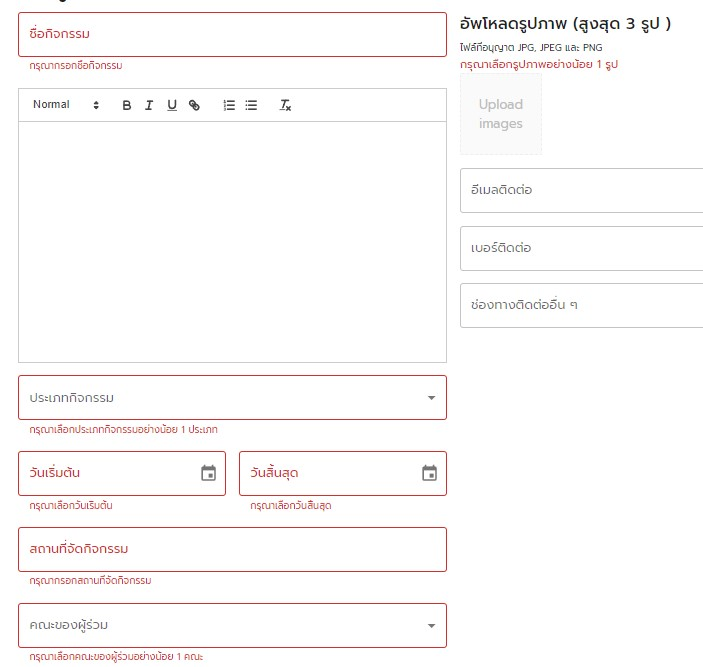
\includegraphics[scale=0.7]{public/required-new.jpg}}
    \end{center}
    \caption[ผลทดลองข้อมูลที่จำเป็นต้องกรอก]{ข้อมูลที่จำเป็นต้องกรอกในหน้าสร้างกิจกรรม}
    \label{fig:create-required}
\end{figure}
\subsubsection{ผลลัพธ์การประกาศกิจกรรม}
เมื่อทดลองการประกาศกิจกรรม โดยใช้ข้อมูลดังนี้
\begin{itemize}
    \item ชื่อกิจกรรม: CMU Library Training
    \item ประเภทกิจกรรม: การพัฒนาตนเอง, วิชาการ
    \item วันเริ่มต้น: 28 ต.ค. 2567 20:30
    \item วันสิ้นสุด: 29 ต.ค. 2567 18:00
    \item สถานที่จัดกิจกรรม: คณะแพทยศาสตร์
    \item คณะของผู้เข้าร่วม: ทุกคณะ
    \item รูปภาพ: จำนวน 3 รูป
\end{itemize}
จะได้ผลลัพธ์ดังต่อไปนี้
\begin{figure}[H]
    \begin{center}
    \fbox{
\includegraphics[scale=0.7]{public/test-create-box.png}}
    \end{center}
    \caption[ผลทดลองข้อมูลรายละเอียดย่อยของกิจกรรมตัวอย่าง]{รายละเอียดย่อยของกิจกรรมตัวอย่าง}
    \label{fig:test-create-box}
\end{figure}
\begin{figure}[H]
    \begin{center}
    \fbox{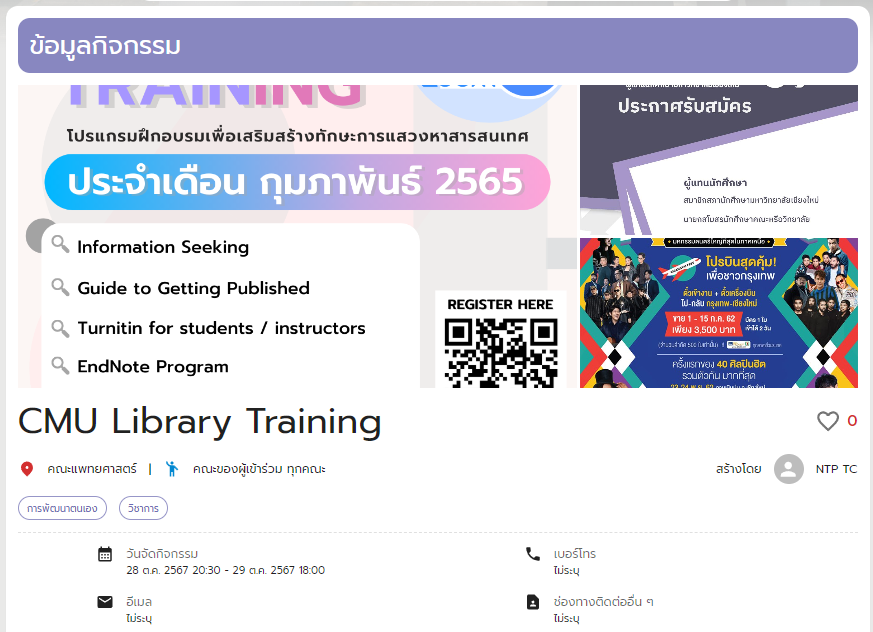
\includegraphics[scale=0.5]{public/test-create-detail.png}}
    \end{center}
    \caption[ผลทดลองข้อมูลรายละเอียดทั้งหมดของกิจกรรมตัวอย่าง]{รายละเอียดทั้งหมดของกิจกรรมตัวอย่าง}
    \label{fig:test-create-detail}
\end{figure}
\subsection{การแสดงความสนใจเข้าร่วมกิจกรรม}
ในหน้ารายละเอียดทั้งหมดของกิจกรรม จะมีปุ่มรูปหัวใจอยู่ เมื่อผู้ใช้กดปุ่มนี้ จะถือว่าผู้ใช้รายนั้นกดสนใจกิจกรรมนี้ แล้วกิจกรรมนี้จะไปปรากฎที่หน้ากิจกรรมของฉัน ในส่วนกิจกรรมที่สนใจ

โดยเมื่อทดลองกดสนใจกิจกรรมในรูปที่ 4.11 แล้วจะได้ผลลัพธ์ดังนี้
\begin{figure}[H]
    \begin{center}
    \fbox{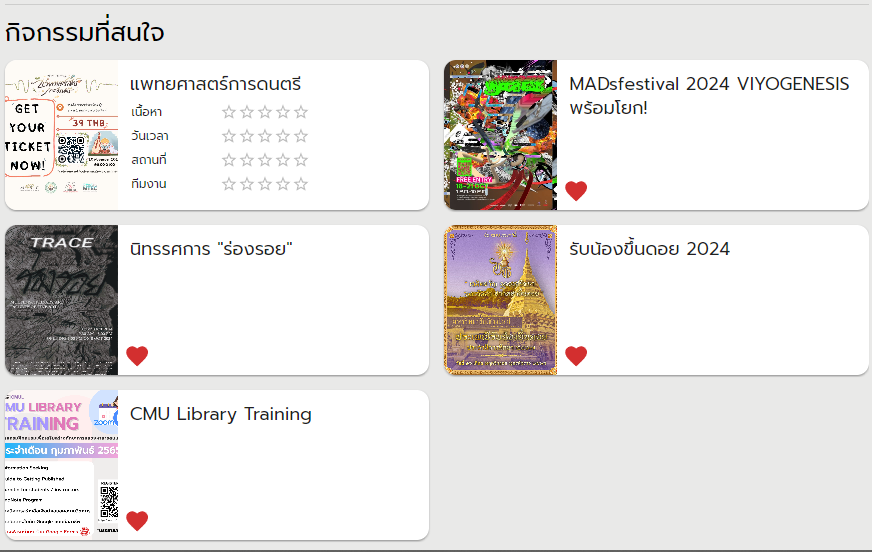
\includegraphics[scale=0.5]{public/test-interest.png}}
    \end{center}
    \caption[ผลทดลองผลลัพธ์การเพิ่มกิจกรรมที่สนใจ]{ผลลัพธ์การเพิ่มกิจกรรมที่สนใจ}
    \label{fig:test-interest}
\end{figure}
\subsection{การเปรียบเทียบวันที่ปัจจุบันและวันเริ่มต้นกิจกรรม}
ในหน้ารายละเอียดย่อยของกิจกรรม ที่มุมขวาบนจะมีการแสดงข้อความเพื่อบ่งบอกว่ากิจกรรมนี้ใกล้มาถึงหรือยัง โดยแบ่งผลลัพธ์เป็น 3 แบบ ดังนี้
\begin{itemize}
    \item กิจกรรมยังไม่เริ่ม: จะแสดงข้อความว่าเหลืออีกกี่วัน ก่อนที่จะเริ่มกิจกรรม
    \item กิจกรรมที่เริ่มแล้วแต่ยังไม่สิ้นสุด: จะแสดงข้อความว่า เริ่มไปแล้ว
    \item กิจกรรมสิ้นสุดแล้ว: จะแสดงข้อความว่า จบไปแล้ว
\end{itemize}
\begin{figure}[H]
    \begin{minipage}[b]{0.48\textwidth}
        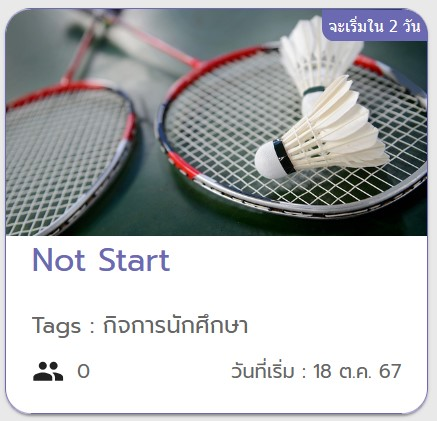
\includegraphics[width=\textwidth, height=5cm]{public/not-start.jpg}
        \caption[ผลทดลองกิจกรรมที่ยังไม่เริ่ม]{ผลลัพธ์กิจกรรมที่ยังไม่เริ่ม}
    \end{minipage}
    \hfill
    \begin{minipage}[b]{0.48\textwidth}
        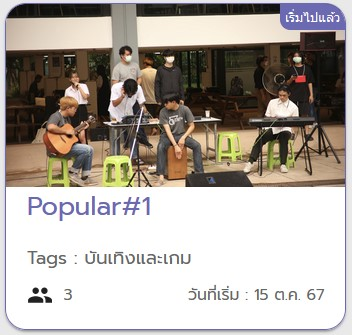
\includegraphics[width=\textwidth, height=5cm]{public/already-started.jpg}
        \caption[ผลทดลองกิจกรรมที่เริ่มไปแล้ว]{ผลลัพธ์กิจกรรมที่ยังไม่สิ้นสุด}
    \end{minipage}
\end{figure}
\begin{figure}[H]
    \begin{center}
    \fbox{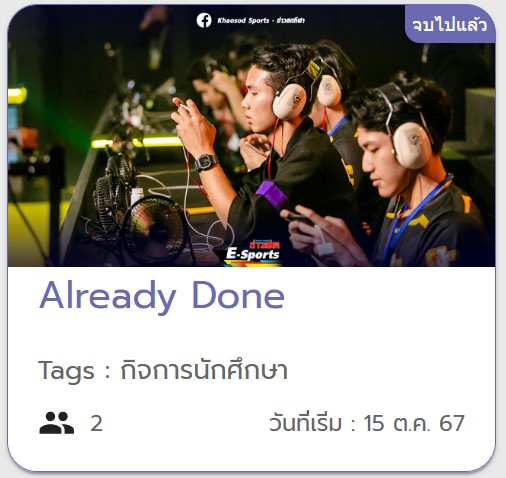
\includegraphics[scale=0.6]{public/already-ended.jpg}}
    \end{center}
    \caption[ผลทดลองกิจกรรมที่สิ้นสุดแล้ว]{ผลลัพธ์กิจกรรมที่สิ้นสุดแล้ว}
    \label{fig:already-ended}
\end{figure}
\section{ผลการทดสอบระบบให้คะแนนกิจกรรม}
\subsection{การอนุญาตสิทธิ์ให้คะแนนกิจกรรม}
ในหน้ากิจกรรมของฉัน ส่วนกิจกรรมที่สนใจ จะแบ่งการแสดงผลเป็น 3 ประเภท คือ 
\begin{itemize}
    \item กิจกรรมที่ยังไม่สิ้นสุด: จะยังไม่สามารถให้คะแนนได้(ในตัวอย่างคือกิจกรรม นิทรรศกาล"ร่องรอย")
    \item กิจกรรมที่สิ้นสุดแล้ว แต่ยังไม่ได้ให้คะแนน: จะแสดงดาวสีขาว บ่งบอกว่ายังไม่ได้ให้คะแนน(ในตัวอย่างคือกิจกรรม คอนเสิร์ต และ แพทยศาสตร์การดนตรี)
    \item กิจกรรมที่สิ้นสุดแล้ว และให้คะแนนแล้ว: จะแสดงผลที่ผู้ใช้เคยให้คะแนนไว้
\end{itemize}
\begin{figure}[H]
    \begin{center}
    \fbox{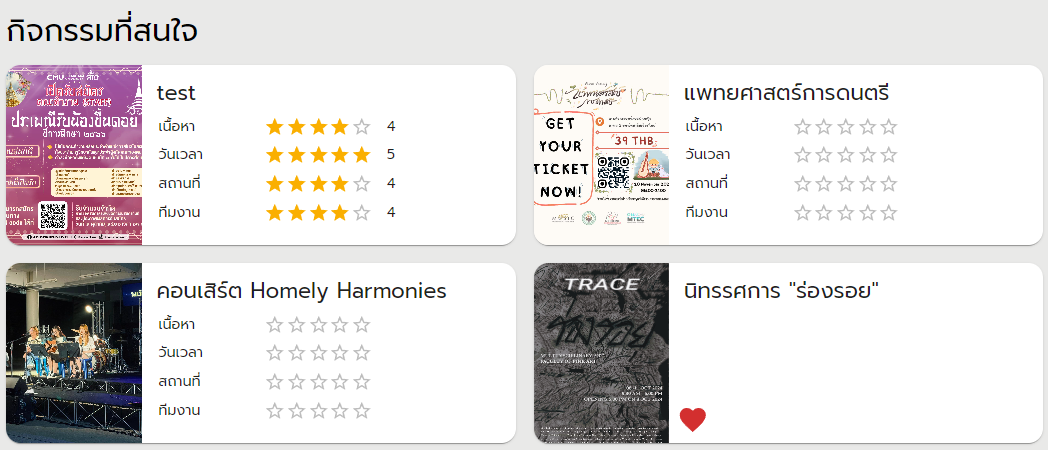
\includegraphics[scale=0.6]{public/score-section.png}}
    \end{center}
    \caption[ผลทดลองการแสดงผลส่วนกิจกรรมที่สนใจ]{การแสดงผลส่วนกิจกรรมที่สนใจ}
    \label{fig:score-section-2}
\end{figure}
\clearpage
\subsection{การแสดงค่าเฉลี่ยของคะแนนกิจกรรม}
เมื่อทดลองให้คะแนนกิจกรรมที่มีคะแนนก่อนหน้า คะแนนเฉลี่ยจะเปลี่ยนไป ดังนี้
\begin{itemize}
    \item เนื้อหา: จากเดิมมี 4 คะแนน เมื่อให้คะแนนใหม่ 3 คะแนน จะได้คะแนนเฉลี่ยเป็น 3.5 คะแนน
    \item วันเวลา: จากเดิมมี 5 คะแนน เมื่อให้คะแนนใหม่ 3 คะแนน จะได้คะแนนเฉลี่ยเป็น 4 คะแนน
    \item สถานที่: จากเดิมมี 4 คะแนน เมื่อให้คะแนนใหม่ 3 คะแนน จะได้คะแนนเฉลี่ยเป็น 3.5 คะแนน
    \item ทีมงาน: จากเดิมมี 5 คะแนน เมื่อให้คะแนนใหม่ 3 คะแนน จะได้คะแนนเฉลี่ยเป็น 4 คะแนน
\end{itemize}
\begin{figure}[H]
    \begin{minipage}[b]{0.48\textwidth}
        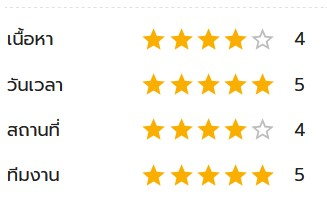
\includegraphics[width=\textwidth,keepaspectratio]{public/after-score-1st.jpg}
        \caption[ผลทดลองคะแนนเฉลี่ยก่อนหน้า]{คะแนนเฉลี่ยก่อนหน้า}
    \end{minipage}
    \hfill
    \begin{minipage}[b]{0.48\textwidth}
        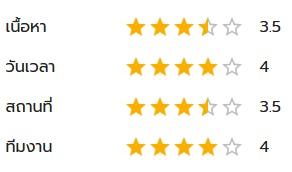
\includegraphics[width=\textwidth,keepaspectratio]{public/after-score-2nd.jpg}
        \caption[ผลทดลองคะแนนเฉลี่ยภายหลัง]{คะแนนเฉลี่ยภายหลัง}
    \end{minipage}
\end{figure}
\subsection{การแสดงหน้าแดชบอร์ด}
จากการทดลอง พบว่าหน้าแดชบอร์ดสามารถดึงข้อมูลจากฐานข้อมูลเพื่อมาแสดงผลในรูปแบบของกราฟได้
\begin{figure}[H]
    \begin{center}
    \fbox{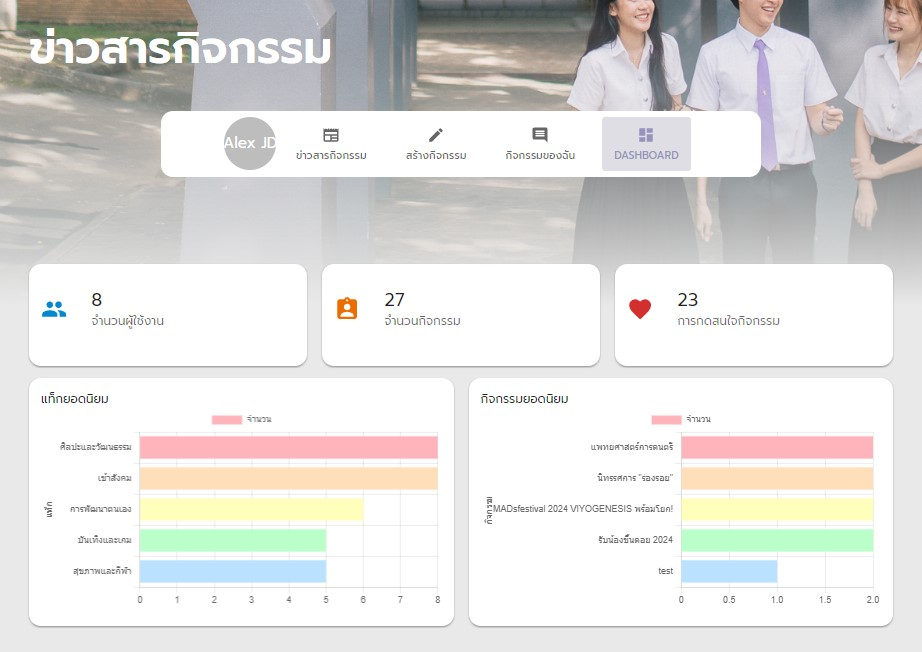
\includegraphics[scale=0.6]{public/dash-page.jpg}}
    \end{center}
    \caption[ผลทดลองการแสดงหน้าแดชบอร์ด]{การแสดงหน้าแดชบอร์ด}
    \label{fig:score-section-2}
\end{figure}
